\section{Introduction to Inductors}
\label{lab_inductors}

%\makelabheader %(Space for student name, etc., defined in master.tex)

\bigskip

\begin{enumerate}[wide]

\item Use your DMM to measure the inductance (in Henries) of several of the inductors in your kits.  You should have eight of them to choose from.  What can you deduce about the color code for the bands?

\item An inductor is basically a series of wire loops, usually around an iron or ferrite core.  Your transformer consists of four sets of wire loops around a common iron core: two primaries and two secondaries.  Make a prediction: which has a greater inductance: one of the primaries (say, white and black leads) or one of the secondaries (say, red and yellow).  Test your prediction.
\begin{center}
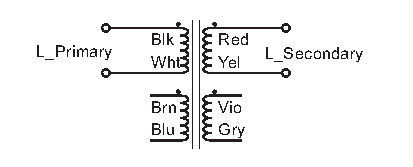
\includegraphics{inductors/transformer_as_inductor1.eps}
\end{center}

\item Make another prediction: given what you just measured for the inductance of one of the primaries, what value do you predict for the inductance of both primaries connected in series, as shown.  Test whether your prediction was correct, and explain why it wasn't. 
\begin{center}

\includegraphics{inductors/transformer_as_inductor2.eps}
\end{center}
 
\medskip 

\textit{Note: For the remainder of this lab, set both of your probes to $10\times$ to minimize the effects of probe capacitance. Also, be sure both channels of your oscilloscope are set to DC coupling.}

\item Build the circuit shown below, with channels 1 and 2 of your scope hooked up as shown, using the two transformer primaries in series as your inductor.  Note that the switch is kind of funny here in that it shorts out the power supply.  To measure the voltage across the resistor $V_{R1}$, you will need to push the ``math'' button on your scope to get it to display the difference Ch2 $-$ Ch1.  It's hard to get the switch to open and close cleanly every time; for best results, try to slide the switch quickly but silently.  Sketch graphs of $V_{R1}$ and $V_L$ versus time both for when you open the switch and for when you close it.   Also sketch the current $I$ vs. time.  What is the time constant $\tau$ of this circuit?  (It should be in the neighborhood of about a millisecond.)  \label{part_rl_constant}
\begin{center}
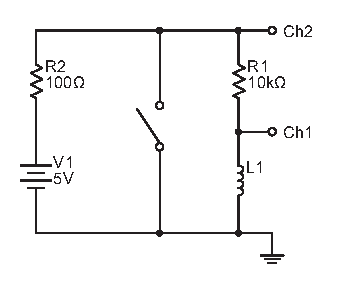
\includegraphics{inductors/single_dc_inductor.eps}
\end{center}

\item Sanity check: Does $V_{R1} +V_L = 5$ volts when the switch is open?  What's $V_{R1} +V_L$ when the switch is closed?

\item In the water pipe analogy, we can think of power supplies as pumps, resistors as constrictions in the pipes, and a capacitor as a flexible rubber membranes stretched across an enlarged section of pipe.  Draw a picture showing the $RL$ circuit you have just built as a system of water pipes, representing the inductor as a giant, heavy water wheel or turbine on frictionless bearings.  
The water flow changes when the pump is turned on or when a valve is opened or closed.
If the mass of the wheel \textit{increases}, does the amount of the water flowing change \textit{more quickly} or \textit{more slowly}?

\item Make a prediction: what will happen to the time constant if you replace $L$ with only a single primary coil of your transformer, instead of two primaries in series?  Check it and see.    

\item Make a prediction: what will happen to the time constant if you replace $R_1$ with a 5~k$\Omega$ resistor?  Check it and see.

\item Figure out a mathematical relationship between $R$, $L$, and the time constant $\tau$.

\item From the graphs of $V_{L}(t)$ and $I(t)$ that you found in part~\ref{part_rl_constant}, can you find an explicit relationship between  $V_{L}(t)$ and $I(t)$?  (Hint: one of them is proportional to the time derivative of the other.  Bonus points if you can find the constant of proportionality.)

\item Compare your answer in the previous part to the situation for the RC circuit you studied in Lab~\ref{lab_capacitors}.  (Remake and remeasure the circuit in part~\ref{part_rc_circuit} of that lab if you don't remember how it worked.)  Make graphs of $V_{C}(t)$ and $I(t)$ as the switch is opened and closed.  Can you find an explicit relationship between $V_{C}(t)$ and $I(t)$, where one of them is proportional to the time derivative of the other?  Again, what's the constant of proportionality?


\end{enumerate}

\textbf{Possible Exam Questions:}

\begin{itemize}
\item The primary of a 10:1 step-down transformer has an inductance of 1.4 Henries.  What is the inductance of the transformer's secondary?

\item An inductor ($L = 35$~mH) and a resistor (200~$\Omega$) are connected in series to a 10~V power supply at time $t = 0$.  Graph the current through the inductor and voltage across the inductor as functions of time.  Find the time at which the voltage across the resistor is 4 volts.

\end{itemize}






